% ----------------------------------------------------------------------
%  Pracovní úkoly
% ----------------------------------------------------------------------
\section{Pracovní úkoly}

\begin{enumerate}
\item Určete rychlost šíření podélných zvukových vln v mosazné tyči metodou Kundtovy trubice. Z naměřené rychlosti zvuku stanovte modul pružnosti v tahu E materiálu tyče.

\item Změřte rychlost zvuku ve vzduchu a v oxidu uhličitém pomocí uzavřeného resonátoru. Výsledky měření zpracujte metodou lineární regrese a graficky znázorněte.

\item Vypočítejte Poissonovu konstantu \( \kappa \) oxidu uhličitého z naměřené rychlosti zvuku.

\end{enumerate}
% ----------------------------------------------------------------------
%  Teoretická část
% ----------------------------------------------------------------------
\section{Teoretická část}

Pro měření rychlosti šíření zvuku oběma způsoby budeme využívat tento vztah

\begin{equation}
    c = \lambda \nu
\end{equation}

kde \( \lambda \) je vlnová délka, \( \nu \) kmitočet a \(c\) rychlost zvuku. Budeme tedy zkoumat průběh stojatého vlnění a pokud dokážeme změřit kmitočet a vlnovou délku, můžeme z toho spočíst hledanou rychlost šíření.

\subsection{Kundtova trubice}
První metoda je založena na názorném odečítání hodnot z průhledné skleněné trubice. Trubice se z jedné strany uzavřena, z druhé strany je do trubice vložena mosazná tyč, u které zkoumáme rychlost šíření zvuku a na jejíž konci je umístěn korek. V trubici je rozprostřena tenká vrstva korkového prášku, který díky zvuku buzeného mosaznou tyčí znázorňuje vlnový průběh. Aparatura je znázorněna na obrázku \ref{fig:kundtova-trubice}.

\begin{figure}[h]
    \centering
    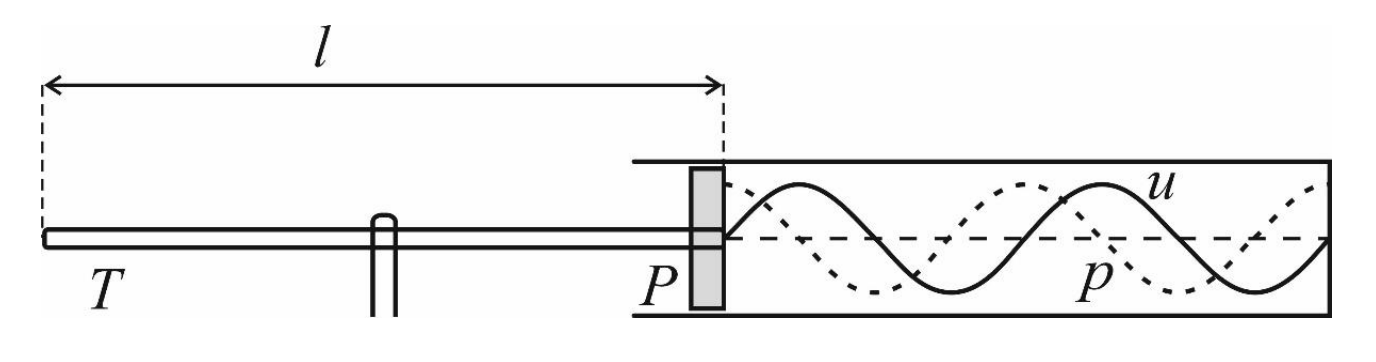
\includegraphics[width=0.6\linewidth]{10 - Rychlost šíření zvuku//Protokol//img/Aparatura Kundtovy trubice.png}
    \caption{Aparatura Kundtovy trubice}
    \label{fig:kundtova-trubice}
\end{figure}

Tyč upevníme uprostřed a tím získáme uzel uprostřed a kmitny na koncích tyče. Proto platí vztah pro vlnovou délku

\begin{equation}
    \lambda = 2l
\end{equation}

Rezonance vznikne, pokud je délka uvnitř trubice rovna celistvému násobku půlvln. Tuto vzdálenost je možné regulovat zasunutím tyče do trubice. Víme, že akustická vlna při přechodu prostředím zachovává svoji frekvenci a proto platí

\begin{equation}
    \frac{c_1}{\lambda_1}=\frac{c_2}{\lambda_2}
\end{equation}

kde \(c_1\) je hledaná rychlost, \(c_2\) rychlost zvuku v trubici (ve vzduchu), \(\lambda_1\) vlnová délka v tyči a \(\lambda_2\) naměřená vlnová délka v trubici. Rychlost \(c_2\) lze určit Laplaceovým vzorcem, abychom ve vztahu (3) redukovali počet neznámých proměnných na jednu

\begin{equation}
    c = \sqrt{\kappa \frac{p}{\rho}}
\end{equation}

kde \(\kappa\) je Poissonova konstanta, \(p\) tlak plynu a \(\rho\) hustota plynu.

V našem případě můžeme rychlost zvuku spočítat ze vzorce pro 50\% vlhkost a teplotu okolo 20 °C

\begin{equation}
    c = [344,36 + 0,63(t - 20 ^{\circ} C)] m \cdot s^{-1}
\end{equation}

Na konec pro určení modulu pružnosti v tahu použijeme rovnici

\begin{equation}
    E = c_1^2 \cdot \rho
\end{equation}

kde \(\rho\) je hustota tyče.

\subsection{Uzavřený rezonátor}

Druhou metodou je využití uzavřeného rezonátoru, který je přesnější avšak méně názorný. Trubice je složena ze dvou souosích trubic, kterým lze regulovat její délku.
Na jedné straně trubice je umístěn generátor zvuku, na kterém lze nastavit přesnou frekvenci. Na druhé straně se nachází mikrofon připojený na voltmetr, kde můžeme hledat maximální výchylky a určit tak hledanou rezonanci. Celá trubice je izolována od okolí s dvěma uzavíratelnými přívody, což umožňuje měřit rychlost v různých plynech. Aparatura je znázorněna na obrázku \ref{fig:uzavreny-rezonator}.

\begin{figure}[h]
    \centering
    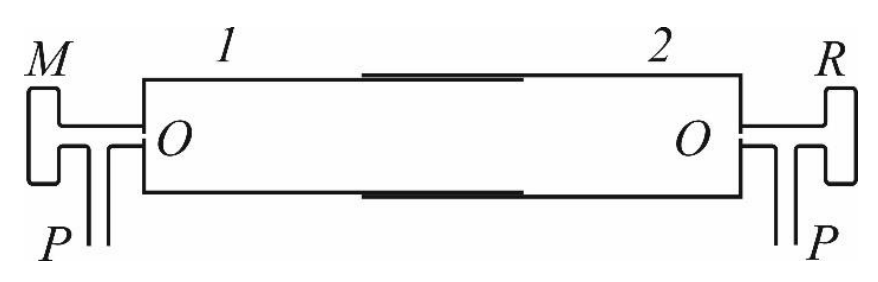
\includegraphics[width=0.6\linewidth]{10 - Rychlost šíření zvuku//Protokol//img/Aparatura uzavřeného rezonátoru.png}
    \caption{Aparatura uzavřeného rezonátoru}
    \label{fig:uzavreny-rezonator}
\end{figure}

Rychlost budeme měřit dvěma způsoby. Prvně nastavíme konstantní délku \(l\) rezonátoru a budeme postupně budeme zvyšovat frekvenci generátoru a pomocí stupnice voltmetru hledat rezonance. Pro tyto rezonance platí vztah

\begin{equation}
    l = k \frac{\lambda_k}{2}
\end{equation}

kde k je přirozené číslo a udává počet půlvln v rezonátoru. Dosazením do (1) získáme

\begin{equation}
    c = \frac{2l \nu_k}{k}
\end{equation}

Úpravou Laplaceova vzorce dostáváme vztah pro ideální plyn

\begin{equation}
    \kappa = \frac{c^2 \mu}{RT}
\end{equation}

kde \(\mu\) je molekulová hmotnost plynu, R molární plynová konstanta a T teplota.
Ve druhém případě necháme konstantní frekvenci a změnou délky l rezonátoru hledáme odpovídající rezonanci. Pro rychlost platí

\begin{equation}
    c = 2(l_1-l_2)\nu
\end{equation}

kde \(l_1-l_2\) je délka mezi dvěma rezonancemi.

% ----------------------------------------------------------------------
%  Výsledky a zpracování měření
% ----------------------------------------------------------------------
\section{Výsledky a zpracování měření}

\subsection{Laboratorní podmínky}

    Měření bylo prováděno za laboratorních podmínek uvedených v tabulce \ref{tab:lab_pod}. 

    \begin{table}[h]
        \centering
        \caption{Laboratorní podmínky}
        \label{tab:lab_pod}
        \begin{tabular}{|c|c|c|} 
        \hline
            t / °C & p / hPa & vlhkost / \%RH  \\ 
        \hline
            23,2(4)   & 959,7(20)   & 35,7(25)            \\
        \hline
        \end{tabular}
    \end{table}

\subsection{Kundtova trubice}
Nejprve bylo třeba zjistit délku mosazné tyče. Měření bylo provedeno třikrát svinovacím metrem s přesností 0,5 mm. Je ale třeba započítat i systematickou chybu 2 mm, která je způsobená tím, že na konci tyče je umístěn korkový píst, který neumožňuje přiložit měřidlo přímo k tyči. Výsledná chyba je spočtena kombinací obou těchto chyb.

\begin{table}[h]
\centering
\caption{Délka mosazné tyče}
\label{tab:delka-tyce}
\begin{tabular}{|c|c|} 
\hline
Číslo měření   & Délka tyče / m  \\ 
\hline
1              & 1,508(2)        \\
2              & 1,508(2)        \\
3              & 1,508(2)        \\ 
\hline
Výsledná délka & 1,508(2)        \\
\hline
\end{tabular}
\end{table}

Odtud lze pomocí vztahu (2) vypočítat vlnovou délku

\begin{equation}
    \nonumber
    \lambda_1 = 3,016(4) \; m
\end{equation}

Pro určení délky zvukové vlny byla svinovacím metrem změřena délka trubice. Opět měříme i se systematickou chybou danou měřením přes trubici.

\begin{table}[h]
\centering
\caption{Délka trubice}
\label{tab:delka-trubice}
\begin{tabular}{|c|c|} 
\hline
Číslo měření   & Délka trubice / m  \\ 
\hline
1              & 0,620(2)          \\
2              & 0,621(2)          \\
3              & 0,620(2)          \\ 
\hline
Výsledná délka & 0,620(2)          \\
\hline
\end{tabular}
\end{table}

Pomocí tyče vybudíme rezonanci. V trubici vidíme 4 půlvlny a můžeme tedy určit vlnovou délku zvuku uvnitř trubice.
Pro určení nejistoty délky trubice byla provedena další měření, kde byla změněna délka trubice a pozorováno, jak to ovlivnilo počet půlvln. Všechny půlvlny byly sledovány při změně délky o 2 cm v obou směrech. Tyto obrazce sice nebyly již tak zřetelné, ale nepřesnost délky byla stanovena právě na 2 cm. Délka trubice při níž se vytváří 4 půlvlny a vlnová délka jsou

\begin{equation}
    \nonumber
    l = 0,62(2) \; m
\end{equation}

\begin{equation}
    \nonumber
    \lambda_2 = 0,31(2) \; m
\end{equation}

Protože naše laboratorní podmínky jsou velmi podobné, můžeme podle (5) vypočítat rychlost šíření

\begin{equation}
    \nonumber
    c_2 = 346,4 \; m \cdot s^{-1}
\end{equation}

Odtud podle (3) získáme rychlost zvuku v tyči

\begin{equation}
    \nonumber
    c_1 = 3368(217) \; m \cdot s^{-1}
\end{equation}

Chyba měření byla stanovena pomocí metody přenosu chyb jako

\begin{equation}
    \nonumber
    \sigma_c_1 = c_1 \sqrt{\frac{\sigma^2_\lambda__1}{\lambda^2_1} + \frac{\sigma^2_\lambda__2}{\lambda^2_2}}
\end{equation}

Hustota mosazné tyče je \(\rho\) = 8600 \(kg \cdot m^3\) a podle (6) je modul pružnosti

\begin{equation}
    \nonumber
    E = 95(13) \; GPa
\end{equation}

kde chyba je rovna

\begin{equation}
    \nonumber
    \sigma_E = 2 \rho c_1 \sigma_c__1
\end{equation}

\subsection{Uzavřený rezonátor}

Základní frekvence rezonátoru byla odhadnuta podle (8) na 214 Hz. V tabulce \ref{tab:rezonanční-frekvence} je vidět, že přesně toto číslo potvrdil i experiment, což znamená, že je to správný odhad a že se v trubici nenachází žádný jiný plyn z předchozích měření. Při konstantní délce rezonátoru l = 0,80(02) m jsme hledali maximální výchylky na voltmetru.

\begin{table}[h]
\centering
\caption{Rezonanční frekvence}
\label{tab:rezonanční-frekvence}
\begin{tabular}{|c|c|c|} 
\hline
k  & \nu_{vzduch} / Hz & \nu_{CO_2} / Hz  \\ 
\hline
1  & 214         & 165       \\
2  & 436         & 342       \\
3  & 650         & 509       \\
4  & 861         & 675       \\
5  & 1073        & 839       \\
6  & 1290        & 1012      \\
7  & 1507        & 1181      \\
8  & 1719        & 1346      \\
9  & 1931        & 1513      \\
10 & 2148        & 1681      \\
\hline
\end{tabular}
\end{table}



% ----------------------------------------------------------------------
%  Diskuse výsledků
% ----------------------------------------------------------------------			
\section{Diskuse výsledků}

% ----------------------------------------------------------------------
%  Závěr
% ----------------------------------------------------------------------
\section{Závěr}
